\documentclass[a4paper,12pt]				{article}
\usepackage[utf8]					{inputenc}
\usepackage[spanish]					{babel}
\usepackage[T1]						{fontenc}
\usepackage[nofontinfo]					{lucidabr}
\usepackage{calc, graphicx}

\usepackage[format    = hang,
	    font      = small,
	    labelfont = bf,
	    labelsep  = endash,
	    width     = .9\textwidth]			{caption}

\usepackage[listofformat=subsimple, format=hang, labelfont=footnotesize,
textfont={it, footnotesize}]				{subfig}

\title{Figuras elaboradas con MetaPost}
\author{José Ramón Gisbert Valls}

\begin{document}


\maketitle{}

\begin{abstract}
	Este documento me permite seguir el aspecto que muestran las
	figuras elaboradas en MetaPost para su inclusión en la memoria al
	ritmo en el que las voy desarrollando.
\end{abstract}

\listoffigures

\clearpage


\begin{figure}
	\begin{center}
		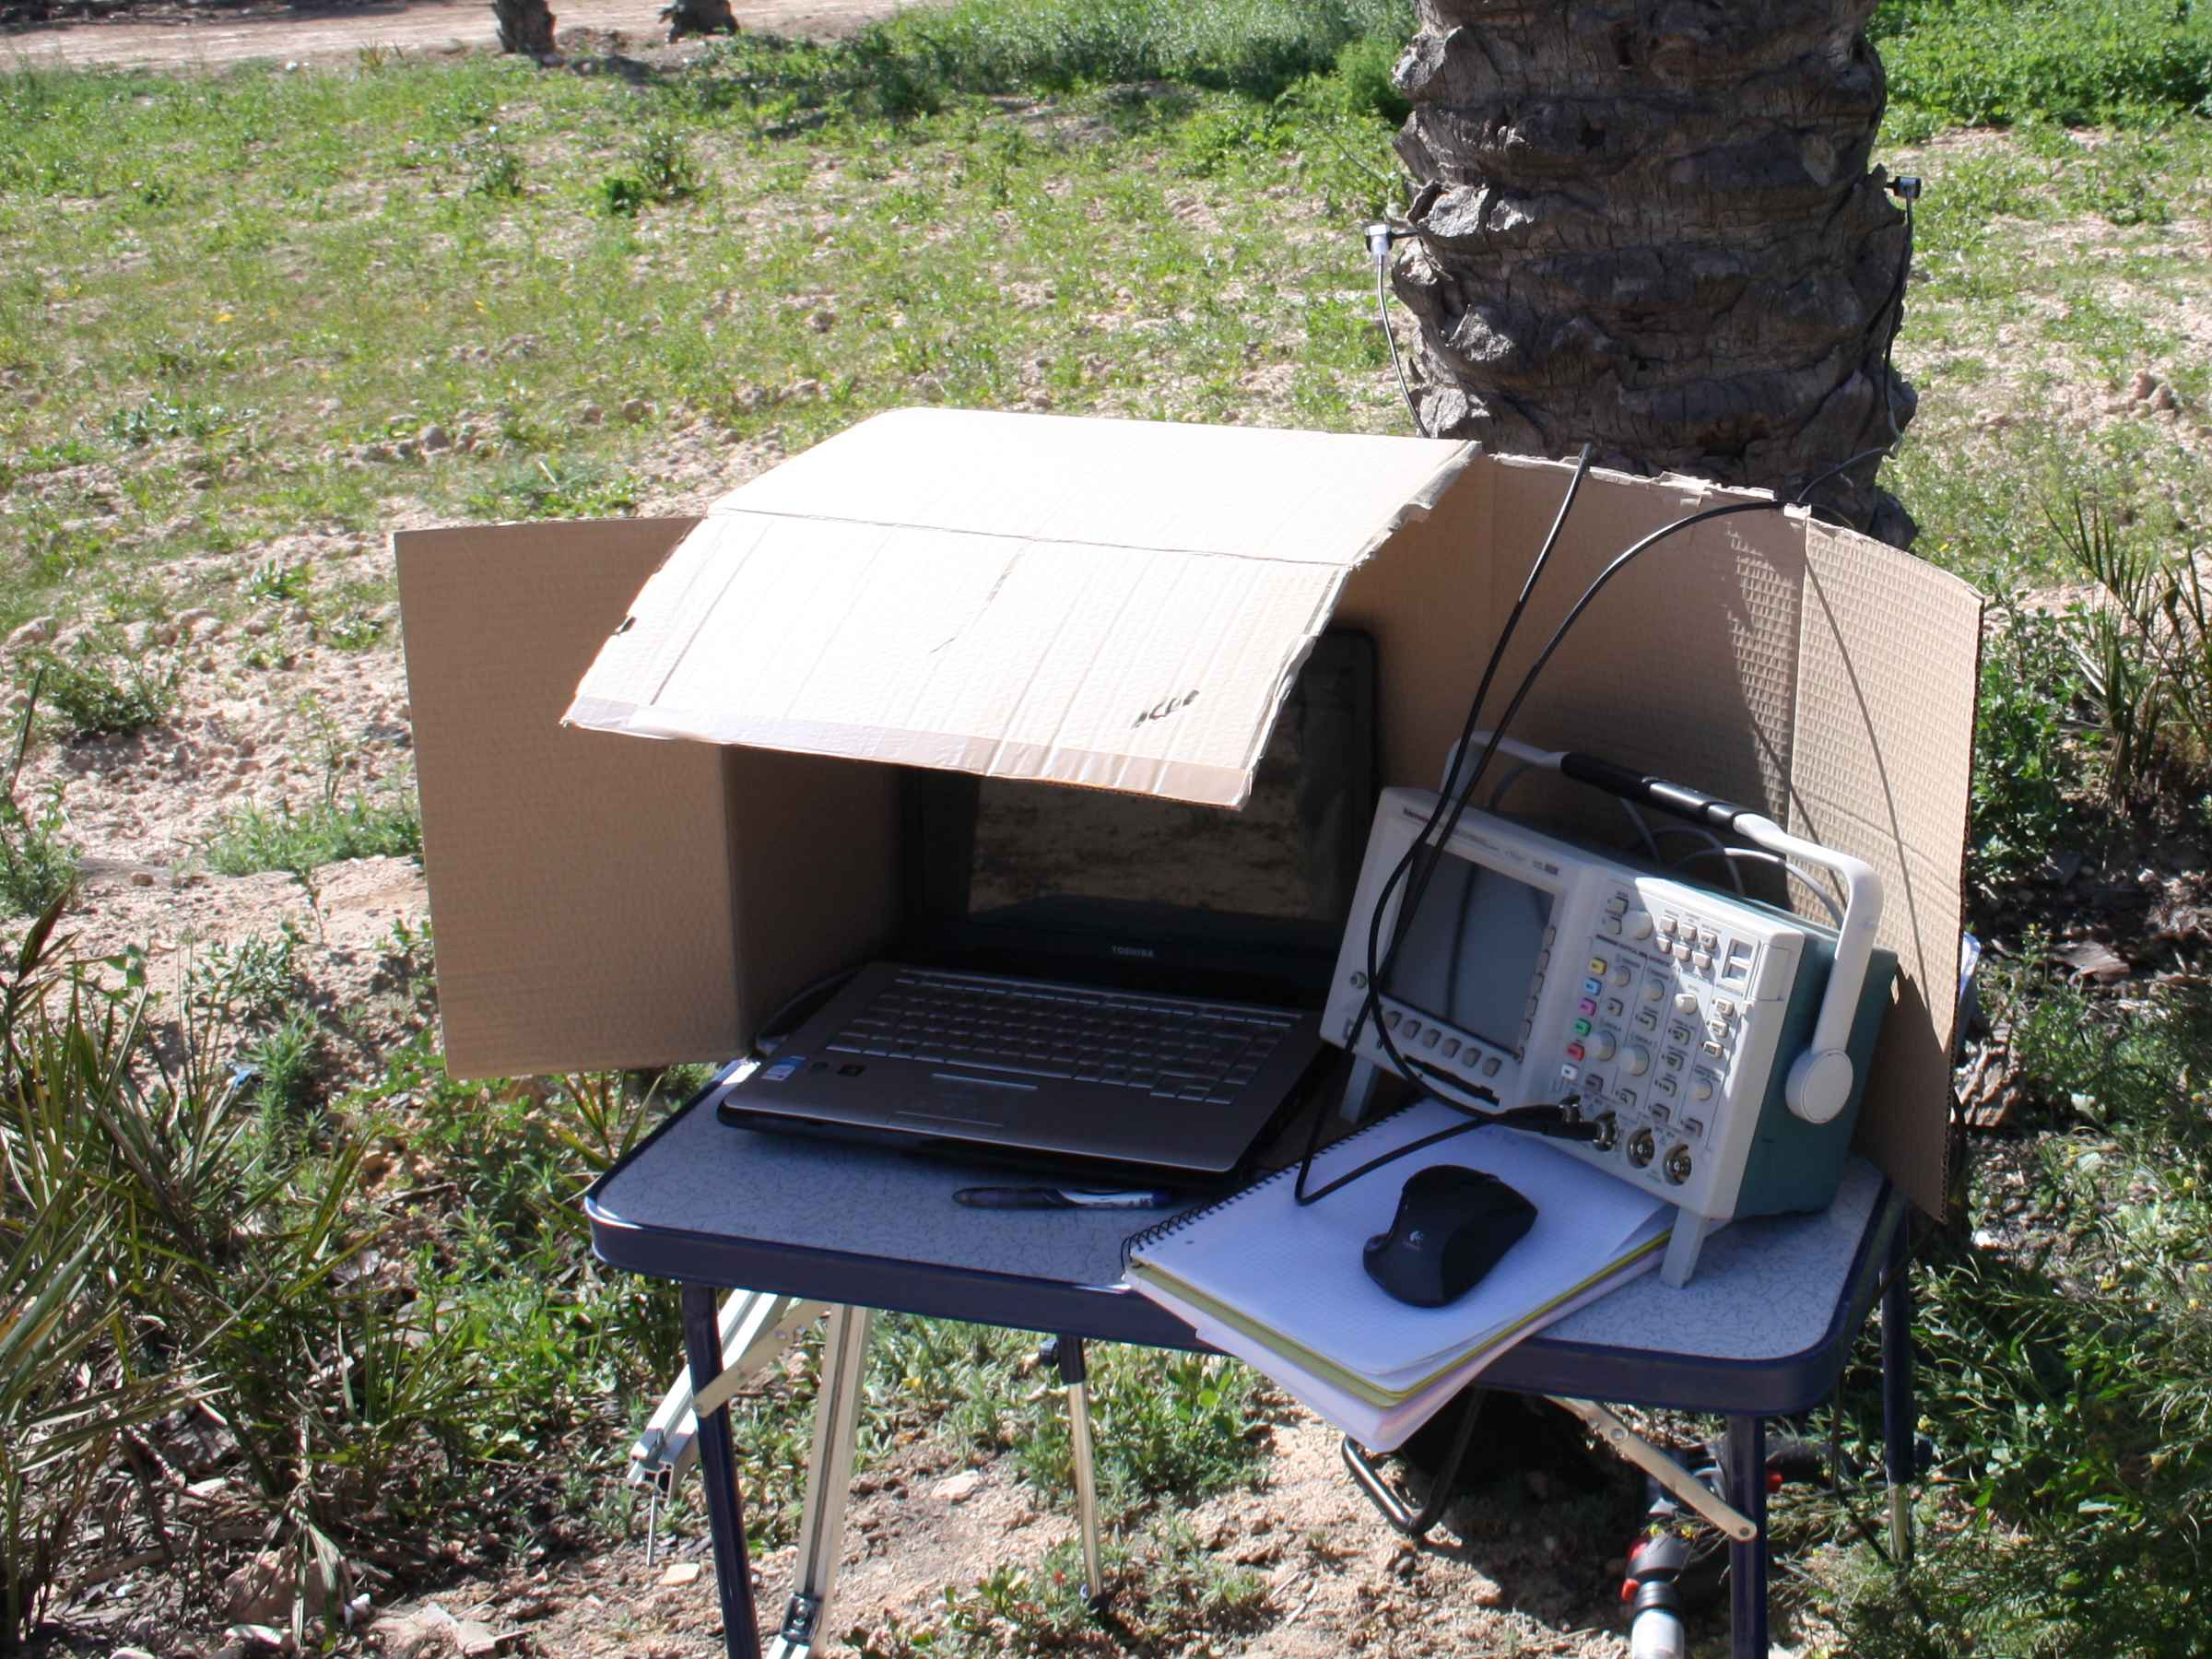
\includegraphics{gis-pfc-ch6-01.pdf}
	\end{center}
	\caption{Gráfico de resultados}
	\label{fig:gis-pfc-ch6-01}
\end{figure}

\begin{figure}
	\begin{center}
		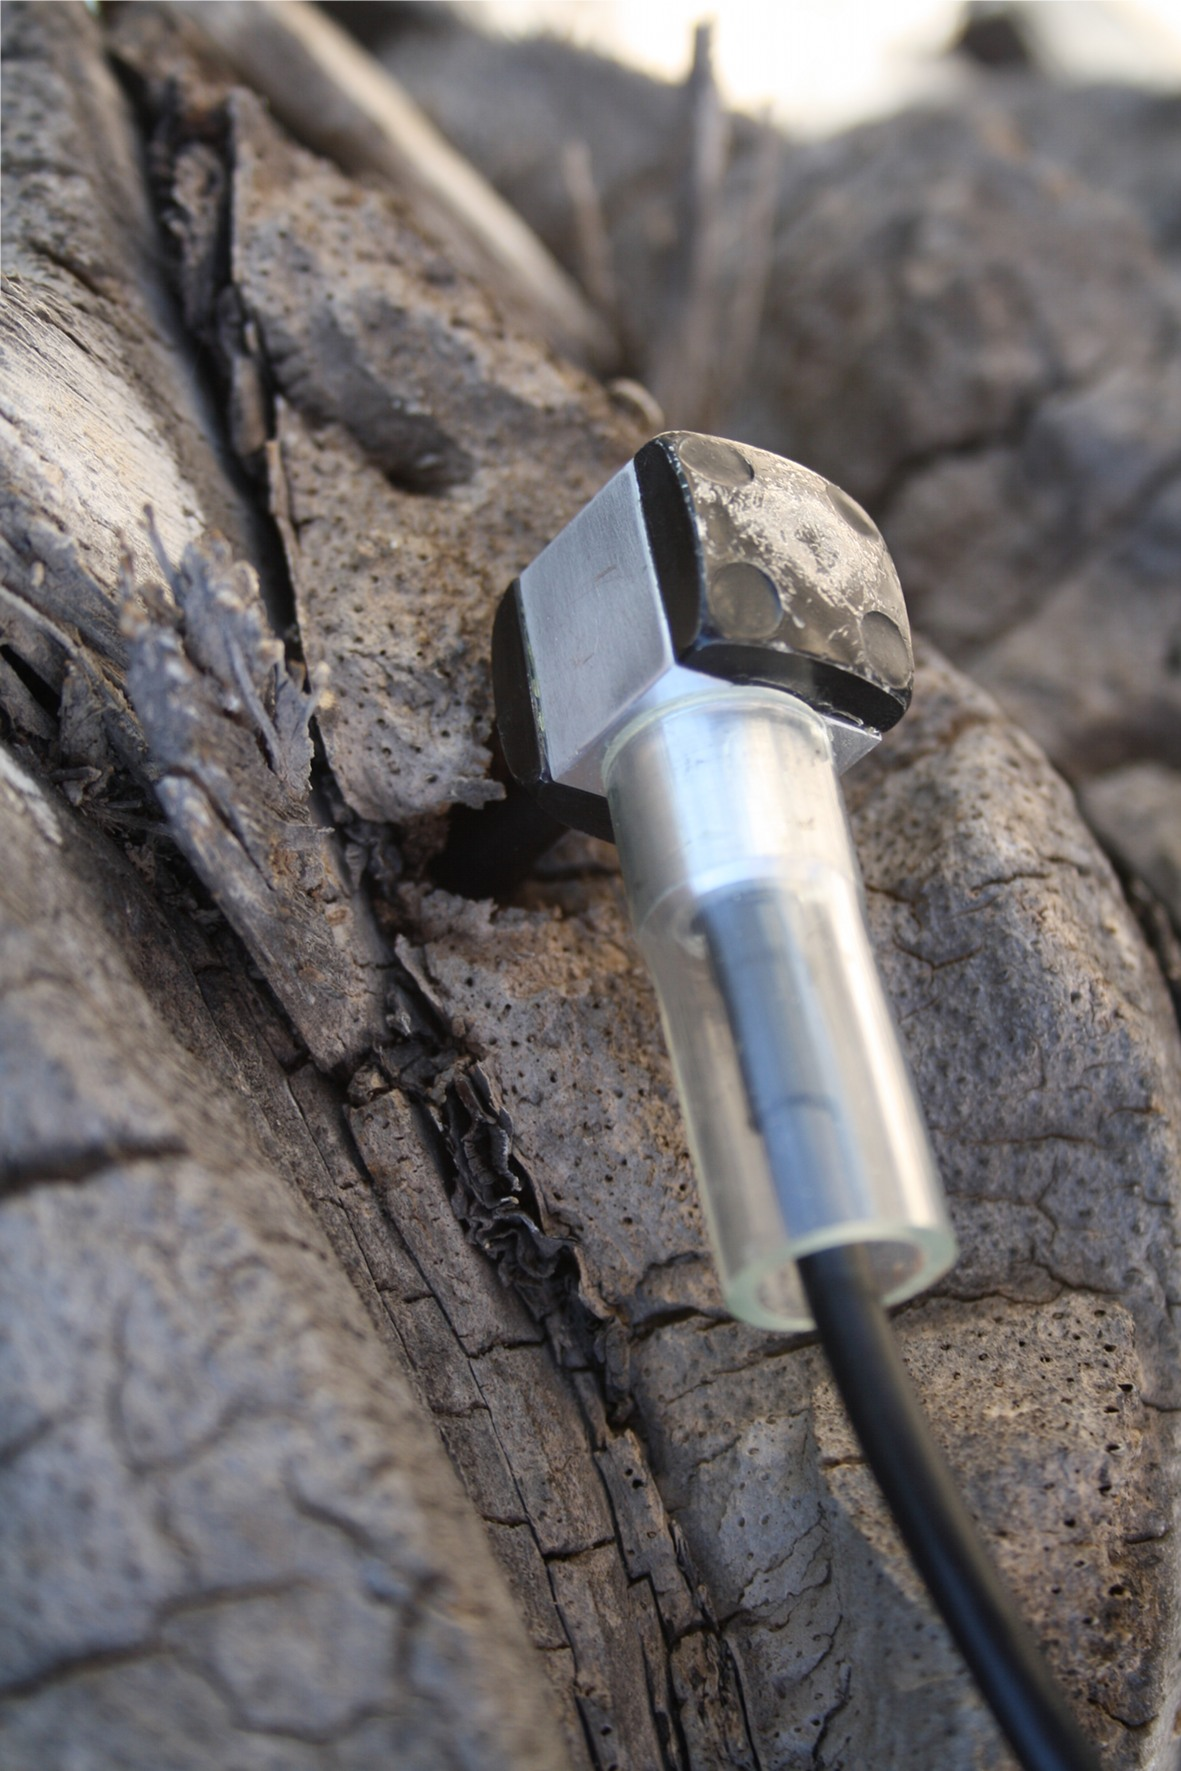
\includegraphics{gis-pfc-ch6-02.pdf}
	\end{center}
	\caption{Gráfico de resultados}
	\label{fig:gis-pfc-ch6-02}
\end{figure}

\begin{figure}
	\begin{center}
		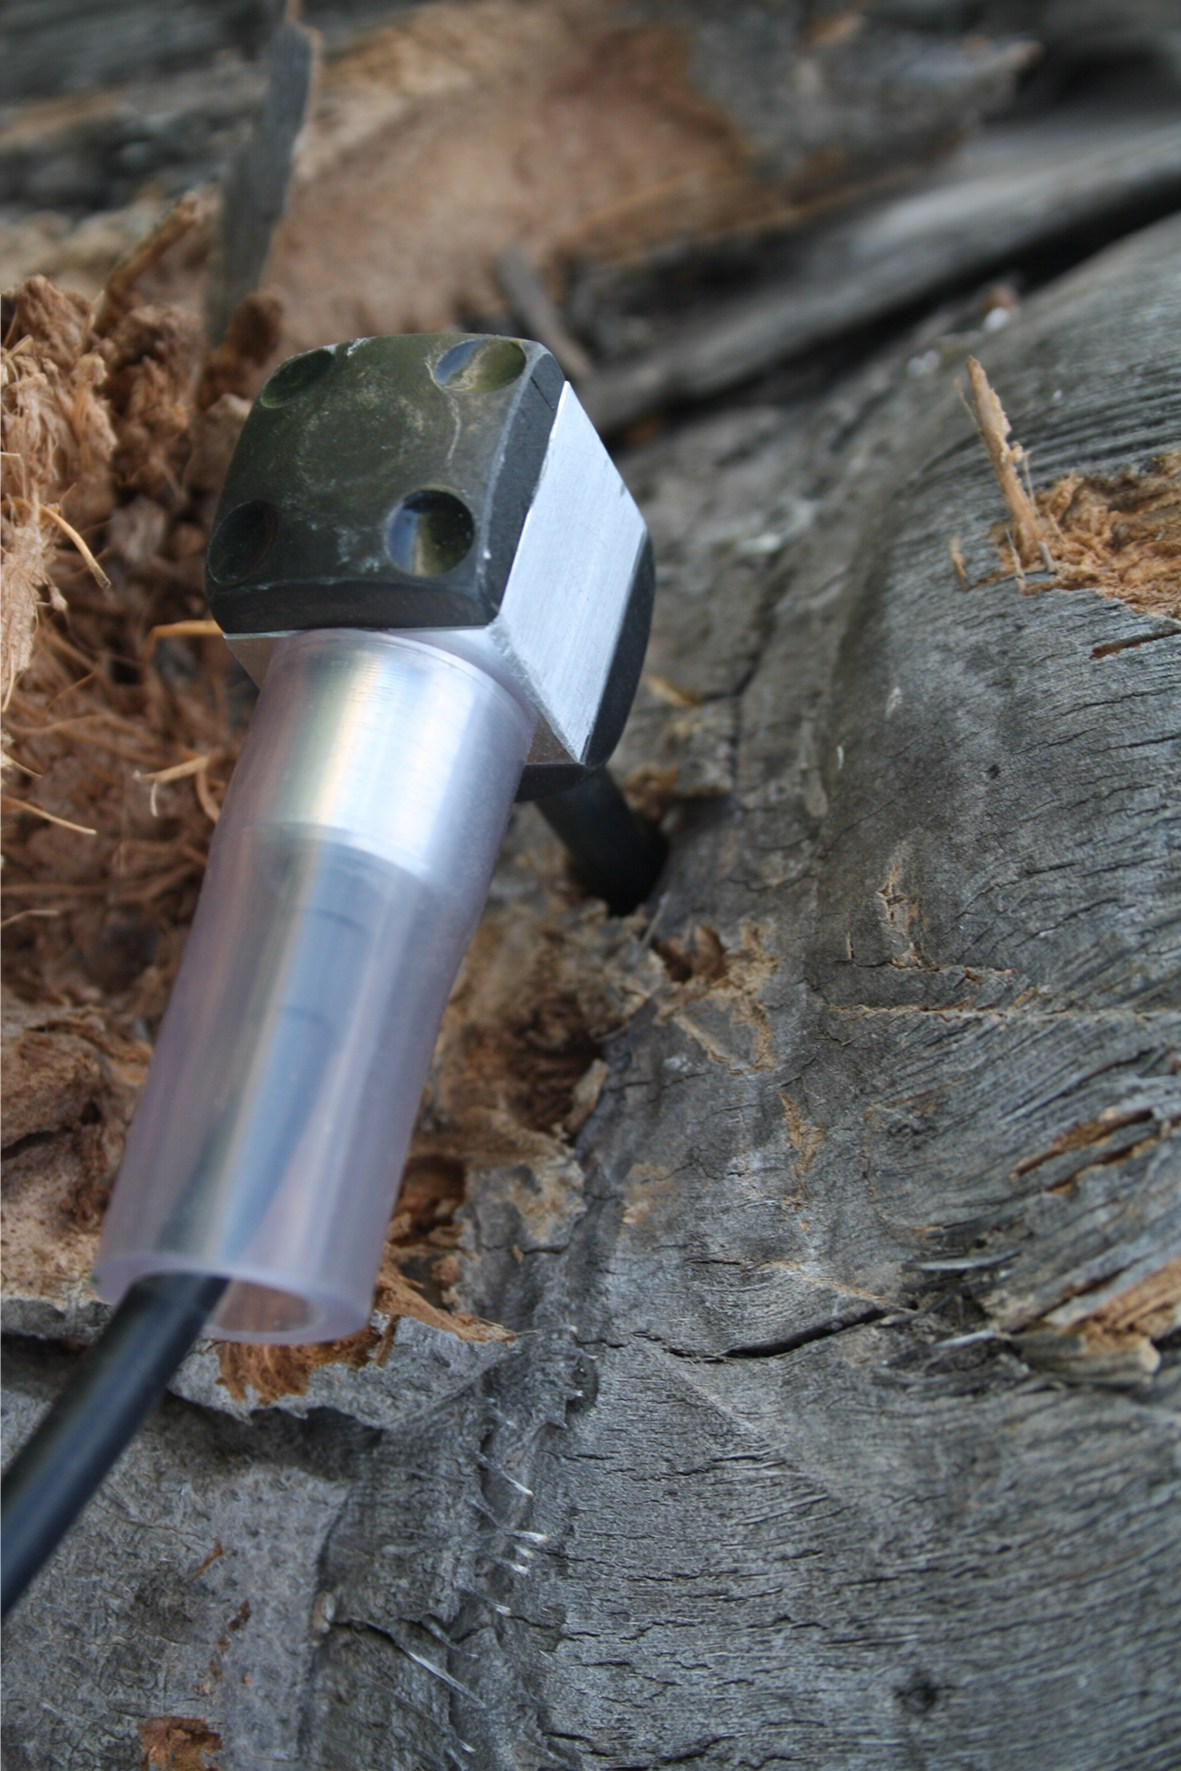
\includegraphics{gis-pfc-ch6-03.pdf}
	\end{center}
	\caption{Gráfico de resultados}
	\label{fig:gis-pfc-ch6-03}
\end{figure}

\begin{figure}
	\begin{center}
		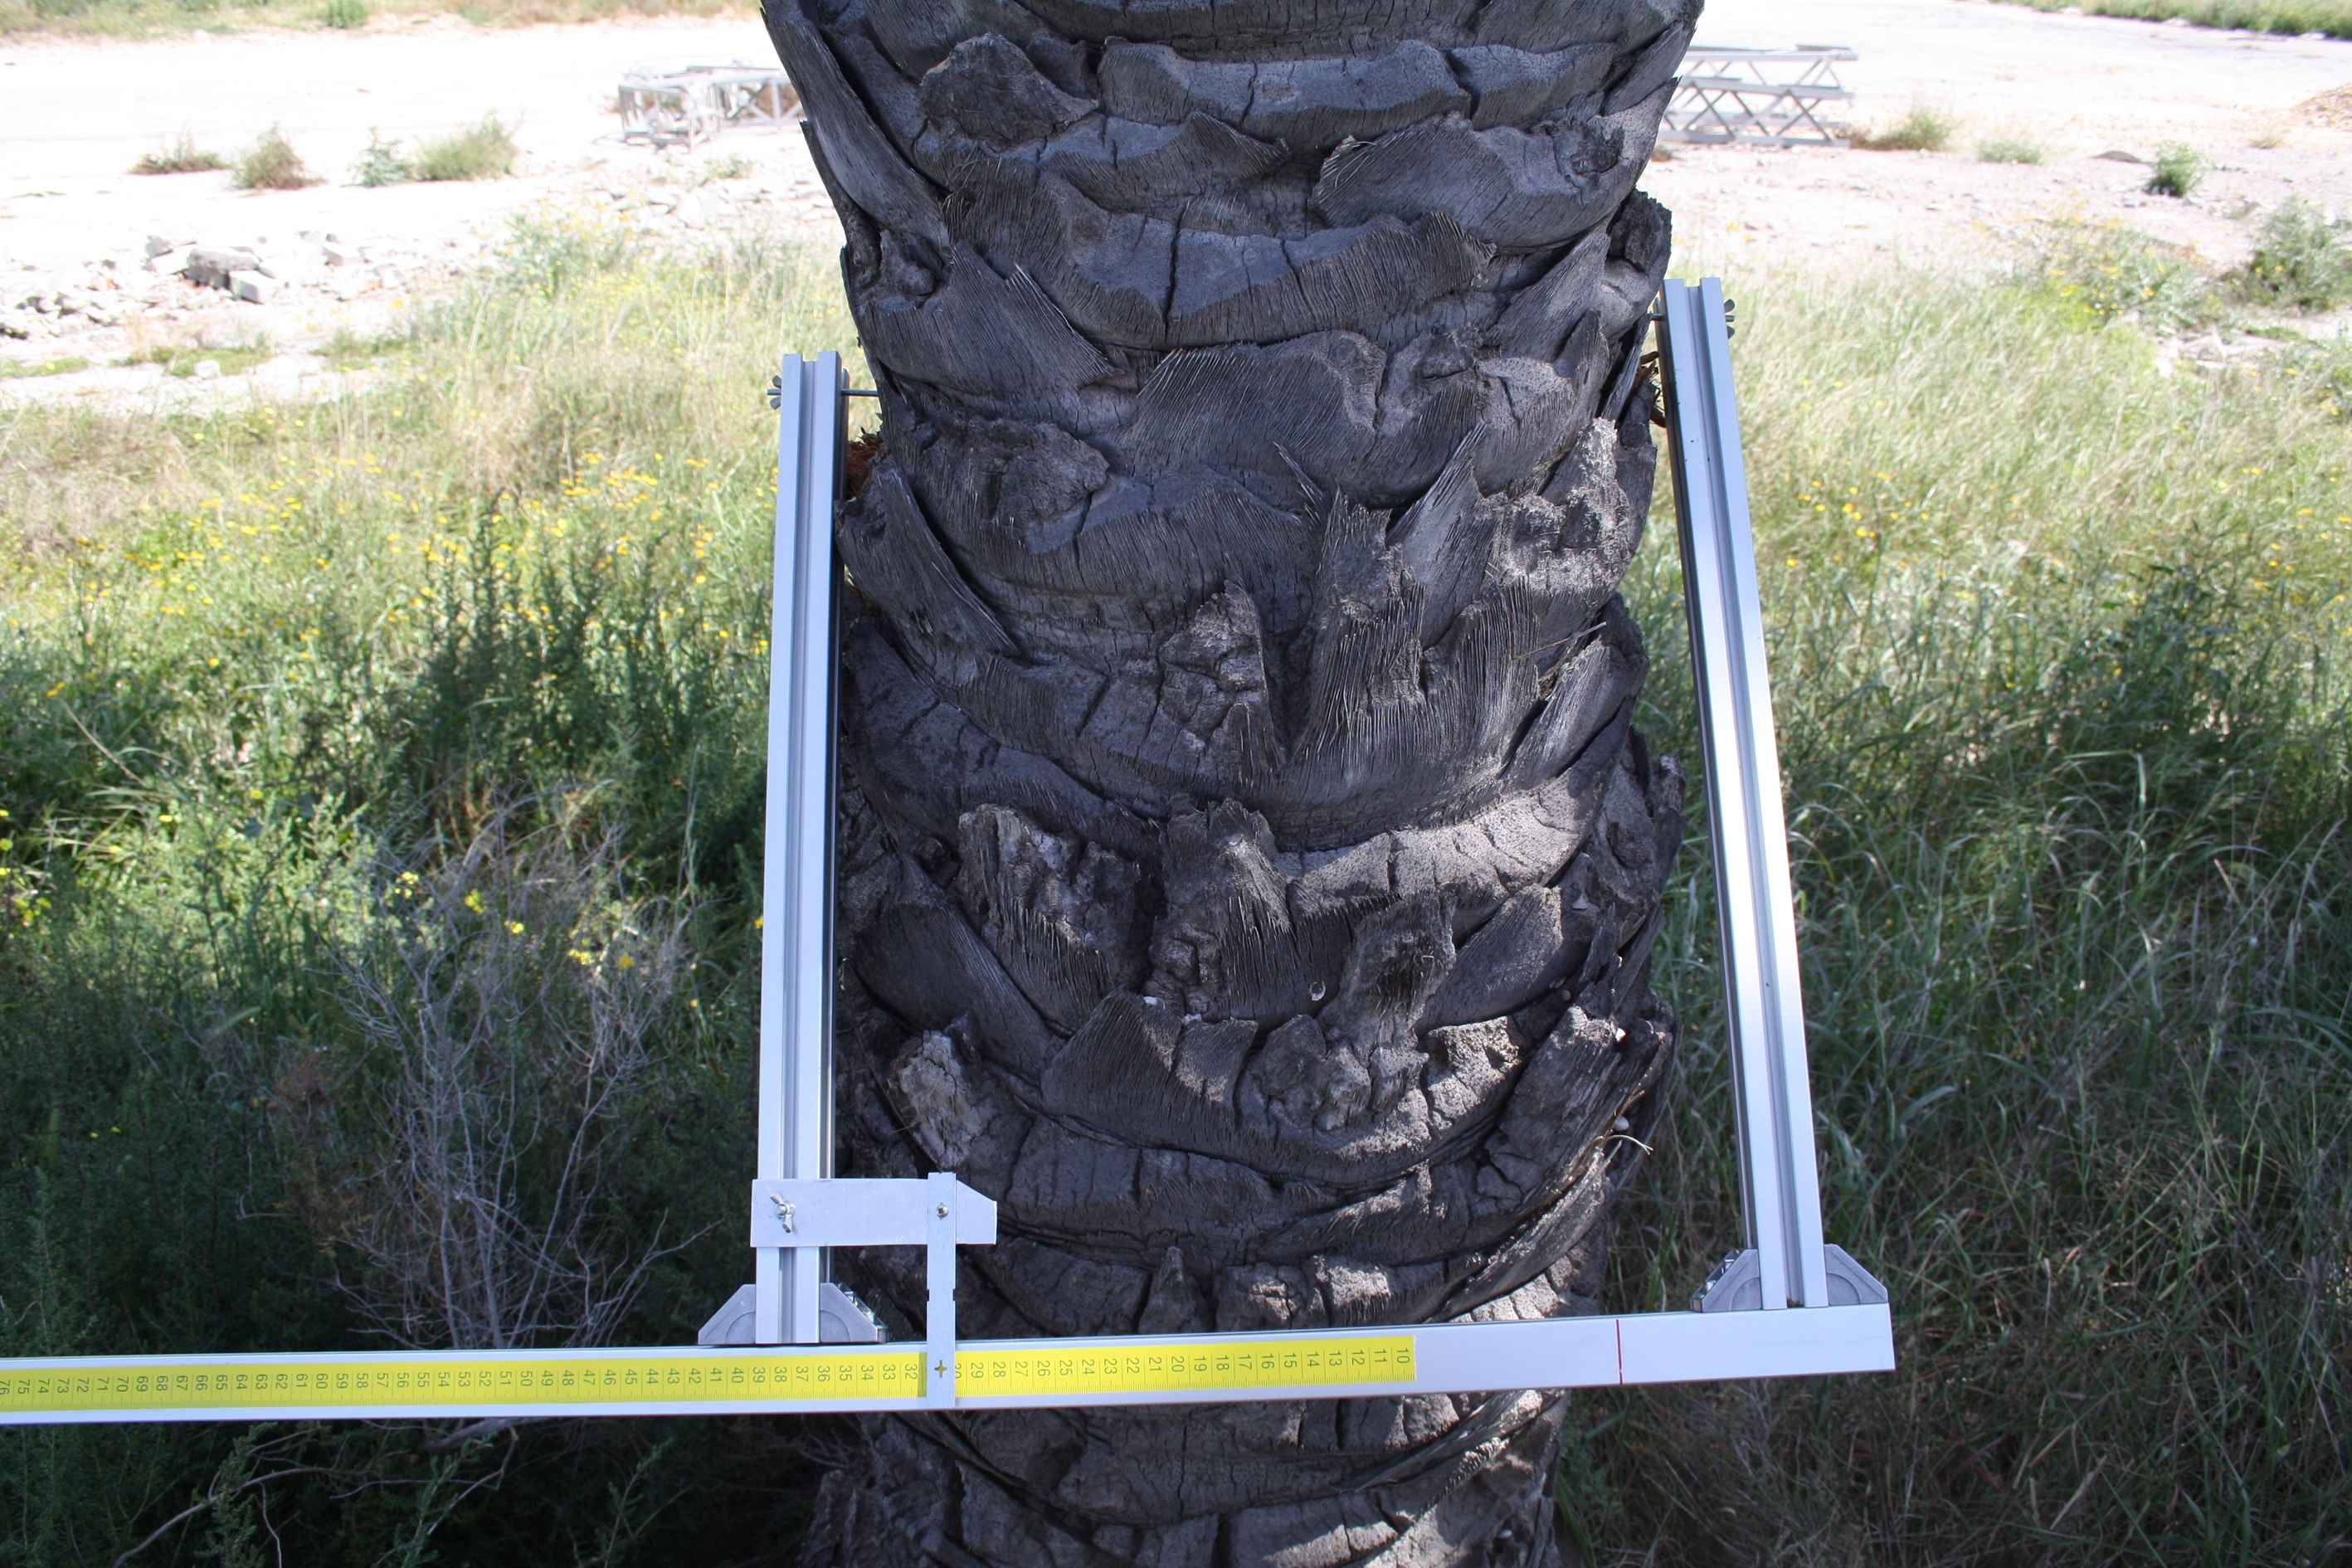
\includegraphics{gis-pfc-ch6-04.pdf}
	\end{center}
	\caption{Gráfico de resultados}
	\label{fig:gis-pfc-ch6-04}
\end{figure}

\begin{figure}
	\begin{center}
		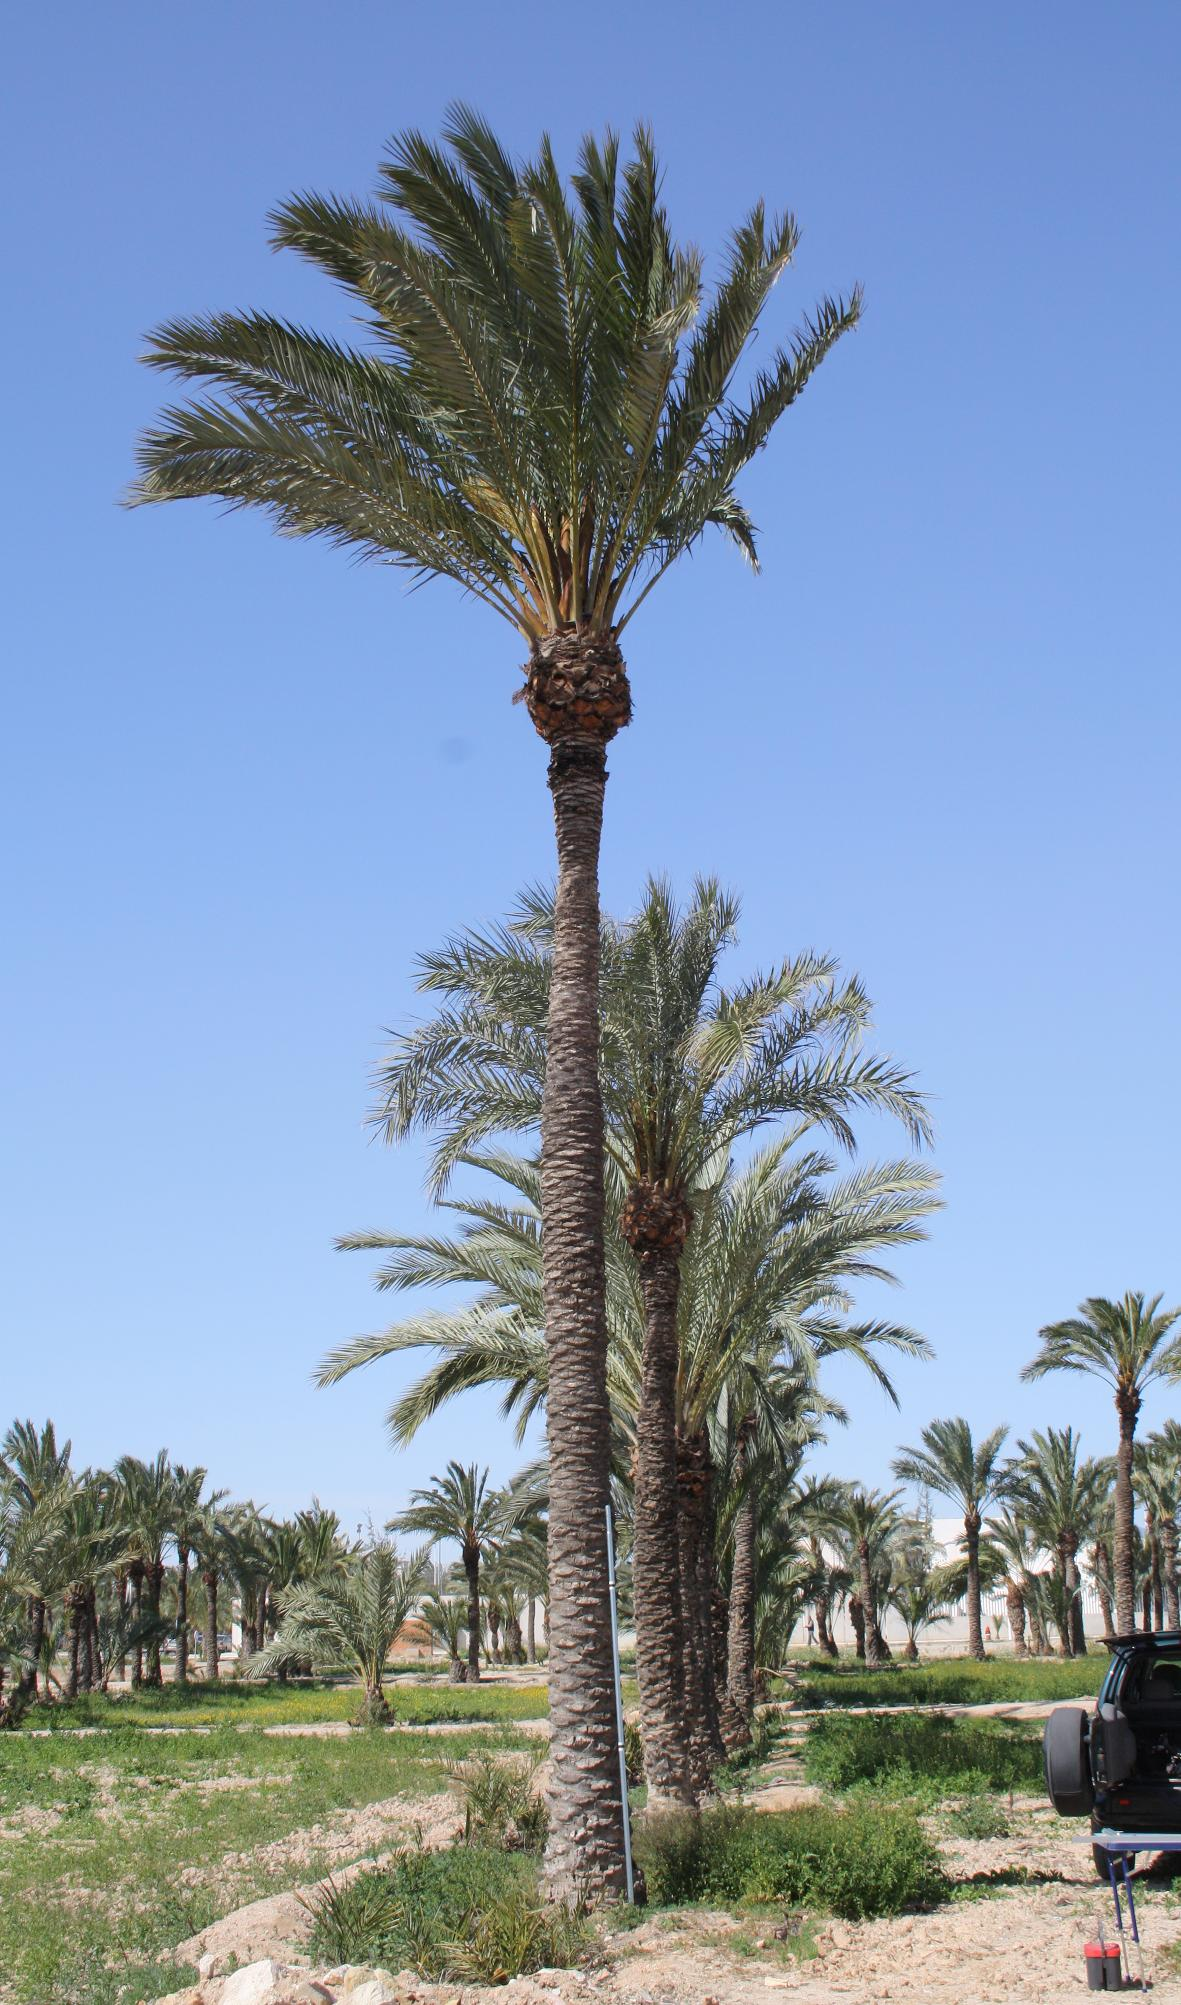
\includegraphics{gis-pfc-ch6-05.pdf}
	\end{center}
	\caption{Gráfico de resultados}
	\label{fig:gis-pfc-ch6-05}
\end{figure}

\begin{figure}
	\begin{center}
		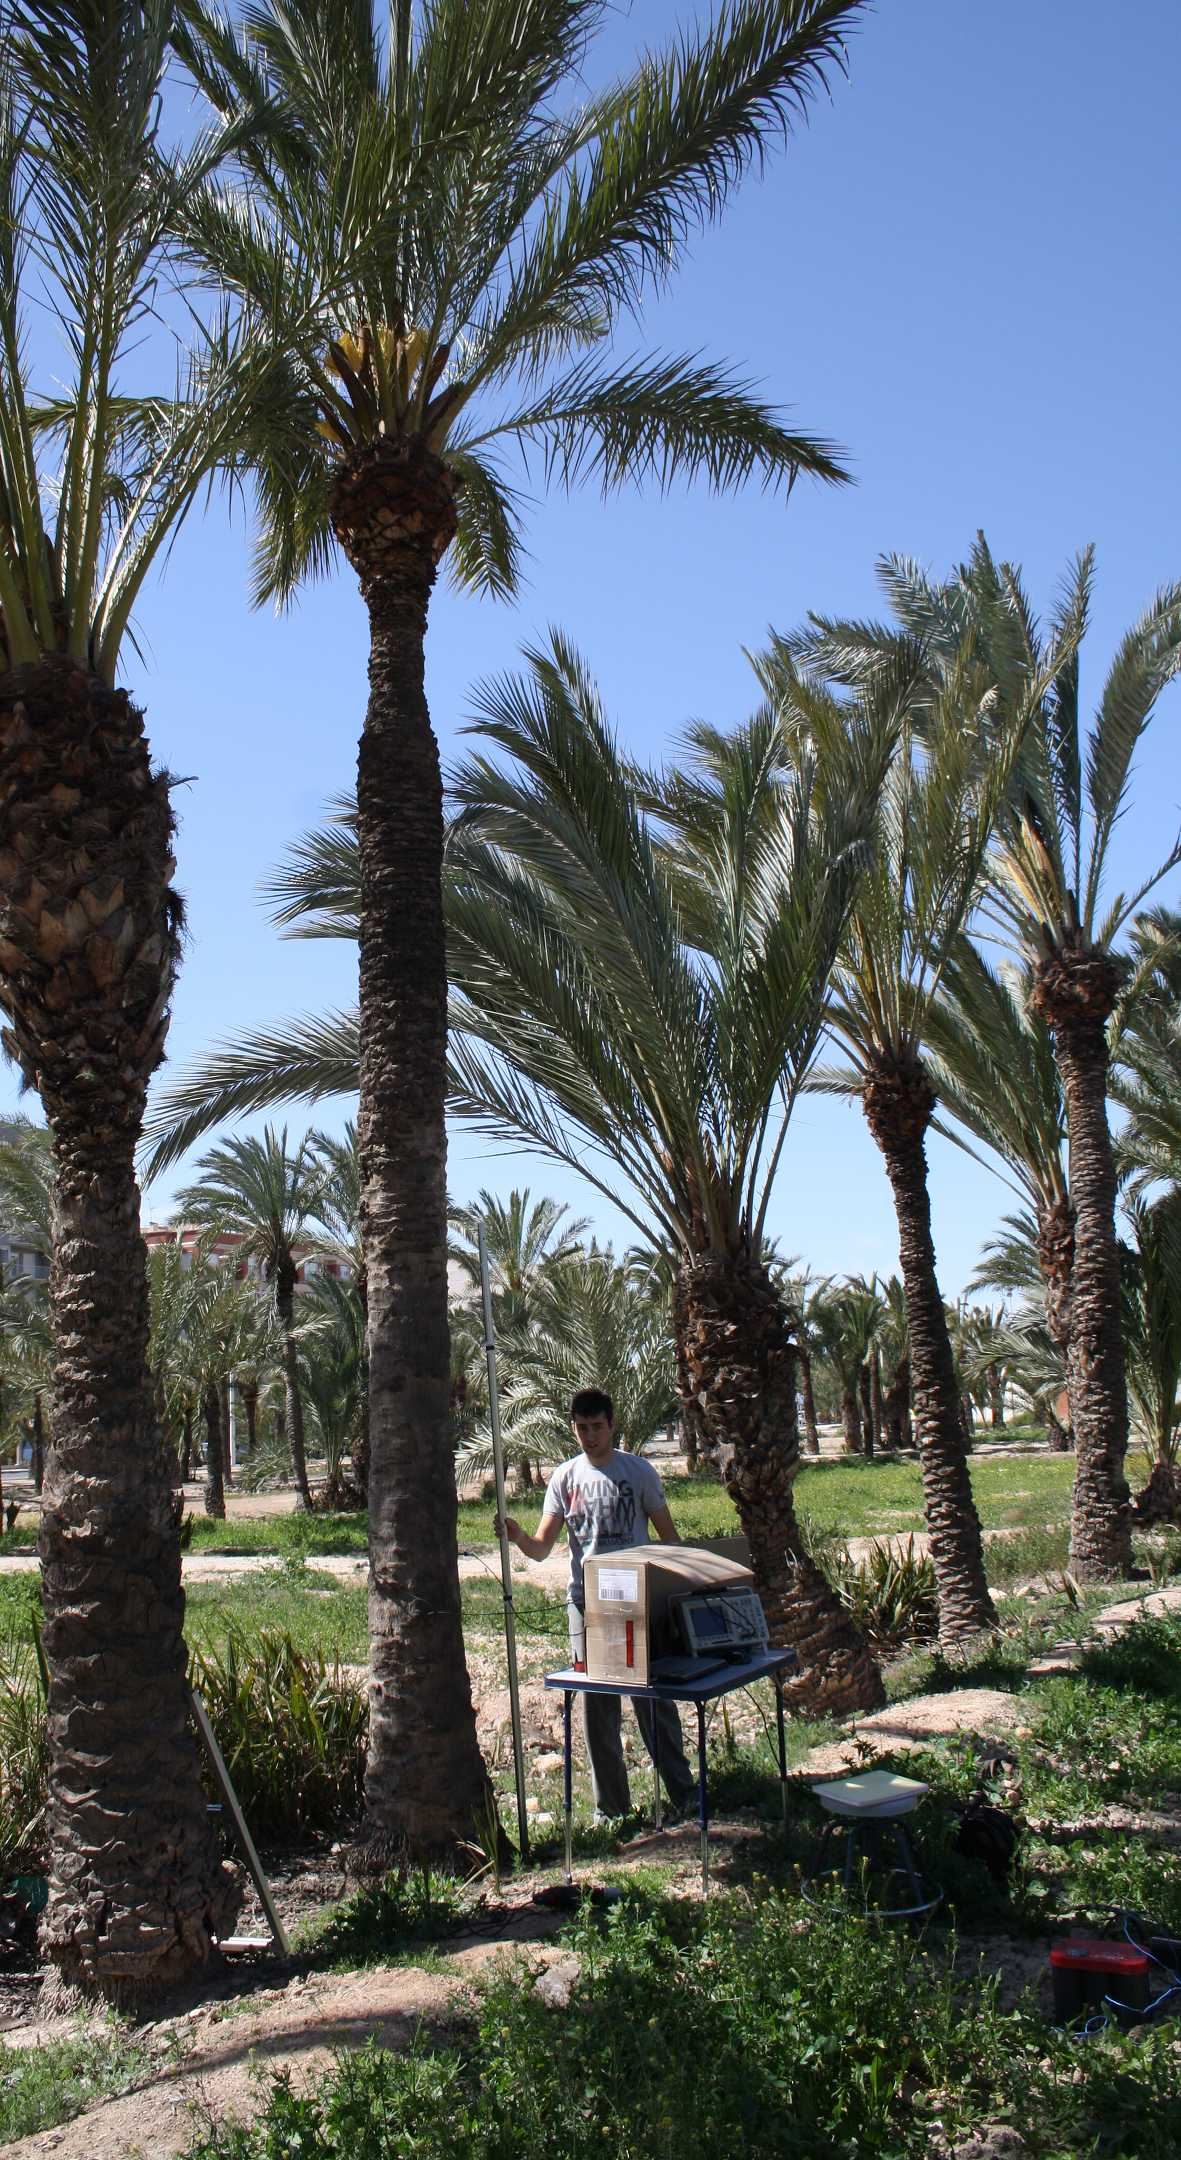
\includegraphics{gis-pfc-ch6-06.pdf}
	\end{center}
	\caption{Gráfico de resultados}
	\label{fig:gis-pfc-ch6-06}
\end{figure}

\begin{figure}
	\begin{center}
		\includegraphics{gis-pfc-ch6-07.pdf}
	\end{center}
	\caption{Gráfico de resultados}
	\label{fig:gis-pfc-ch6-07}
\end{figure}

\begin{figure}
	\begin{center}
		\includegraphics{gis-pfc-ch6-08.pdf}
	\end{center}
	\caption{Gráfico de resultados}
	\label{fig:gis-pfc-ch6-08}
\end{figure}

\begin{figure}
	\begin{center}
		\includegraphics{gis-pfc-ch6-09.pdf}
	\end{center}
	\caption{Gráfico de resultados}
	\label{fig:gis-pfc-ch6-09}
\end{figure}

\begin{figure}
	\begin{center}
		\includegraphics{gis-pfc-ch6-10.pdf}
	\end{center}
	\caption{Gráfico de resultados}
	\label{fig:gis-pfc-ch6-10}
\end{figure}

\end{document}
